\section*{Notations}
We start with some notations we will use along this report.
\begin{itemize}[font= \color{blue} \large, label= $\bullet$]
 \item For any function, $g(\cdot)$ denotes the function $g: x \mapsto g(x)$.
 \item In integrals, $\d x$ denote $\d \lambda(x)$, \ie with respect to the Lebesgue measure.
\end{itemize}

\section*{Introduction}

The goal of the article \cite{FWBQ} is to compute efficiently the integrals of the form
$ \displaystyle \int _ { \X } f ( x ) p ( x ) \mathrm { d } x$
where $\X \subseteq \R ^ { d }$ is a measurable space,
$d \geq 1$ integer representing the dimension of the problem, $p$ a probability
density with respect to the Lebesgue measure on $\X$ and $f : \X \rightarrow \R$
 is a \textit{test}-function.

 We will use the common approximation
 \begin{boxproblem}
   \begin{equation}
  \int _ { \X } f ( x ) p ( x ) \d x \approx \sum _ { i = 1 } ^ { n } w _ { i } f \left( x _ { i } \right)
   \end{equation}
 \end{boxproblem}

 but of course the real challenge lies in the choice of sequences $\acc{x_i}$ and
 $\acc{w_i}$ :
  \begin{mydescription}
    \item [Monte Carlo]: $w_i = \frac{1}{n}$ and $x_i$ realization of multivariate
    random variable $X_i \stackrel{iid}{\sim} X$ where $X$ has $p(\cdot)$ as probability
    distribution.
    \item [Kernel herding]:
    \item [Quasi-Monte Carlo]:


  \item [Frank-Wolfe Bayesian Quadrature]:
  \begin{myitemize}[0.2cm]
\item $\acc{w_i}$ appear naturally in the Bayesian Quadrature by taking the expectation of a posterior distribution  (described in section \ref{sec:BQ}),
\item $\acc{x_i}$ are selected by the Frank-Wolfe algorithm in order to minimize a posterior variance (described in section \ref{sec:FW}).
\end{myitemize}
  \end{mydescription}
  The main interest of the method developed in \cite{FWBQ} is the super fast
  \textit{exponential} convergence to the true value of the integral compared to the other methods mentioned above.\\

\noindent
  Through this report, we will detail every results from \cite{FWBQ} with the goal
  to clarify and explain details that could have been omitted intentionally or not and which, in our view, make the Briol's and al. approach more natural, intuitive and easier
  to understand.
  % use Bach presentation for convergence rates benchmark

\section{Background}
% write $\mu_p$ with an integral
%WHY RKHS, WHY so USEFUL ?
Let $\X \subseteq \R ^ { d }$ be a measurable space, $\mu$ a measure on $\X$ such
that $p = \frac{\d \mu}{ \d \lambda}$ where $\lambda$ denotes the Lebesgue measure on $\X$,
  $\H \subset L^2(\X, \R; \mu)$ be an RKHS with a
 reproducing kernel $k: \X \times \X \rightarrow \R$, $\Phi$ its canonical feature
 map associated. We denote respectively by $\bigps{\cdot}{\cdot}$ and $\norme{\cdot}$
 the bigps product and norm induced on $\H$.

 Recall that the following relations hold:
 \begin{boxexercise}
   \begin{align}
  \forall x \in \X , \quad &k ( \cdot , x ) \in \H\\
  \forall x \in \X , \forall f \in \H , \quad &\langle f , k ( \cdot , x ) \rangle _ { \H } = f ( x )\\
  \forall (x,y) \in \X^2 \quad &k(x,y) = \bigps{\Phi(x)}{\Phi(y)}
  \end{align}
\end{boxexercise}


Let's denote as \cite{FWBQ}:
\begin{boxdefinition}
  \begin{align*}
    p[f] &:= \int _ { \X } f ( x ) \mathrm { d } \mu(x) = \int _ { \X } f ( x ) p ( x ) \mathrm { d } x\\
    \p[f]&:=\sum _ { i = 1 } ^ { n } w _ { i } f \left( x _ { i } \right).
  \end{align*}
\end{boxdefinition}


We will use the \textit{maximum mean discrepancy} (MMD) as our main metric to measure
 the accuracy of the approximation $p[f] \approx \p[f]$ in the worst case scenario and which is defined as
 \begin{boxdefinition}
    $$\MMD : = \sup _ { f \in \H : \norme{f}=1 } | p [ f ] - \hat { p } [ f ] |.$$
 \end{boxdefinition}

 Let's show (formula 3. in \cite{FWBQ}) that MMD can be rewrite as
 \begin{boxtheorem}
   \begin{align}
     \MMD = \left\| \mu _ { p } - \mu _ { \hat { p } } \right\| _ { \mathcal { H } }
   \end{align}
   where $\mu_p(\cdot) = p[\Phi(\cdot)]$ and $\mu_{\p}(\cdot) = \p[\Phi(\cdot)]$.
 \end{boxtheorem}

   \begin{itemize}[leftmargin=*, font= \color{blue} \large, label= $\bullet$]
     \item \textbf{For all $f$ in $\H$, we have $p[f] = \bigps{f}{\mu_p}$.} By using
     the dirac delta function, the continuity of the inner product and viewing integral
     as a limit of a sum, we get
     \begin{boxcomputation}
     \begin{align*}
       p[f] &= \int_{\X} f(x) \d \mu(x)\\
       &= \int_{\X} \delta_x[f]  \d \mu(x)\\
       &= \int_{\X} \bigps{f}{\Phi(x)}  \d \mu(x)\\%TODO Not obvious
       &=  \bigps{f}{\int_{\X} \Phi(x) \d \mu(x)} \\
       &= \bigps{f}{\mu_p}
     \end{align*}
      \end{boxcomputation}
     \item \textbf{For all $f$ in $\H$, we have $\p[f] = \bigps{f}{\mu_{\p}}$.}
     \begin{boxcomputation}
     \begin{align*}
       \p[f] &= \sum_{i=1}^n w_i f(x_i)\\
       &= \sum_{i=1}^n w_i \delta_{x_i}[f]\\
       &= \sum_{i=1}^n w_i \bigps{f}{\Phi(x_i)}\\%TODO Not obvious
       &=  \bigps{f}{\sum_{i=1}^n w_i \Phi(x_i)} \\
       &= \bigps{f}{\mu_{\p}}
     \end{align*}
   \end{boxcomputation}
\item By using previous results and the Cauchy-schwartz inequality, we get :
\begin{boxcomputation}
\begin{align*}
\MMD &= \sup _ { f \in \H : \norme{f} = 1 } \abs{
\bigps{f}{\mu_{p}-\mu_{\p}} }\\
&\leq \sup _ { f \in \H : \norme{f} = 1 } \norme{f} \norme{\mu_{p}-\mu_{\p}}\\
&= \norme{\mu_{p}-\mu_{\p}}
\end{align*}
 \end{boxcomputation}
with equality if and only if $f$ and  $\mu_{p}-\mu_{\p}$ are linearly dependent.
We deduce the desired result by taking $ \displaystyle f = \frac{1}{\norme{\mu_{p}-\mu_{\p}}}\prt{\mu_{p}-\mu_{\p}}$.

   \end{itemize}



% on maximise avec cauchy schwartz + égalité

\section{Bayesian Quadrature}
\label{sec:BQ}
Let's place a functional prior on the integrand $f$ and denote by $(\Omega, \mathcal{F}, \P)$ its probability space associated. We will assume that $f$ to be
 a \textit{centered} \textbf{gaussian process} with the kernel $k$ as its covariance
 function, \ie
 \begin{boxexample}
   \begin{align*}
     \forall x \in \H, \quad  &\Expec{f(x)} = 0\\
     \forall x, y \in \H, \quad  &\Cov{f(x)}{f(y)} = k(x,y)
   \end{align*}
 \end{boxexample}
A useful property is that $p[f]$ is a gaussian variable and then completely defined by its second-order statistics:
\begin{boxtheorem}
  \begin{align}
    \Expec{p[f]} &= 0\\
    \Var{p[f]} &= \int_{\X^2} k(x,y) \d \mu(x) \d \mu(y)
  \end{align}
\end{boxtheorem}


  By switching integrals using Fubini's theorem, we get
  \begin{boxcomputation}
    \begin{align*}
      \Expec{p[f]} &= \int_{\Omega} p[f](w) \d \P(w)\\
      &= \int_{\Omega} \int_{\X} f(x,w) \d \mu(x)  \d \P(w)\\
      &= \int_{\X} \underbrace{\int_{\Omega}  f(x,w) \d \P(w)}_{\Expec{f(x)}=0} \d \mu(x)  =0
    \end{align*}
\end{boxcomputation}
\begin{boxcomputation}
  \begin{align*}
      \Var{p[f]} &= \Expec{p[f]^2} = \int_{\Omega} p[f](w)^2 \d \P(w)\\
      &=\int_{\Omega} \prt{\int_{\X} f(x,w) \d \mu(x)}^2 \d \P(w)\\
      &=\int_{\Omega} \int_{\X^2} f(x,w)f(y,w) \d \mu(x) \d \mu(y) \d \P(w)\\
      &= \int_{\X^2} \underbrace{\int_{\Omega}  f(x,w)f(y,w) \d \P(w)}_{=\Cov{f(x)}{f(y)} = k(x,y)} \d \mu(x) \d \mu(y) \\
      &= \int_{\X^2}  k(x,y) \d \mu(x) \d \mu(y)
    \end{align*}
\end{boxcomputation}

Assume that samples $\acc{x_i}$ and $\acc{f_i} := \acc{f(x_i)}$ are given for $i=1$ to $n$ and denote by $K:= \prt{k(x_i, x_j)}_{1 \leq i,j \leq n}$. A natural question arises: how to update the weights $\acc{w_i}_{i=1}^n $?

\begin{figure}[H]
\centering
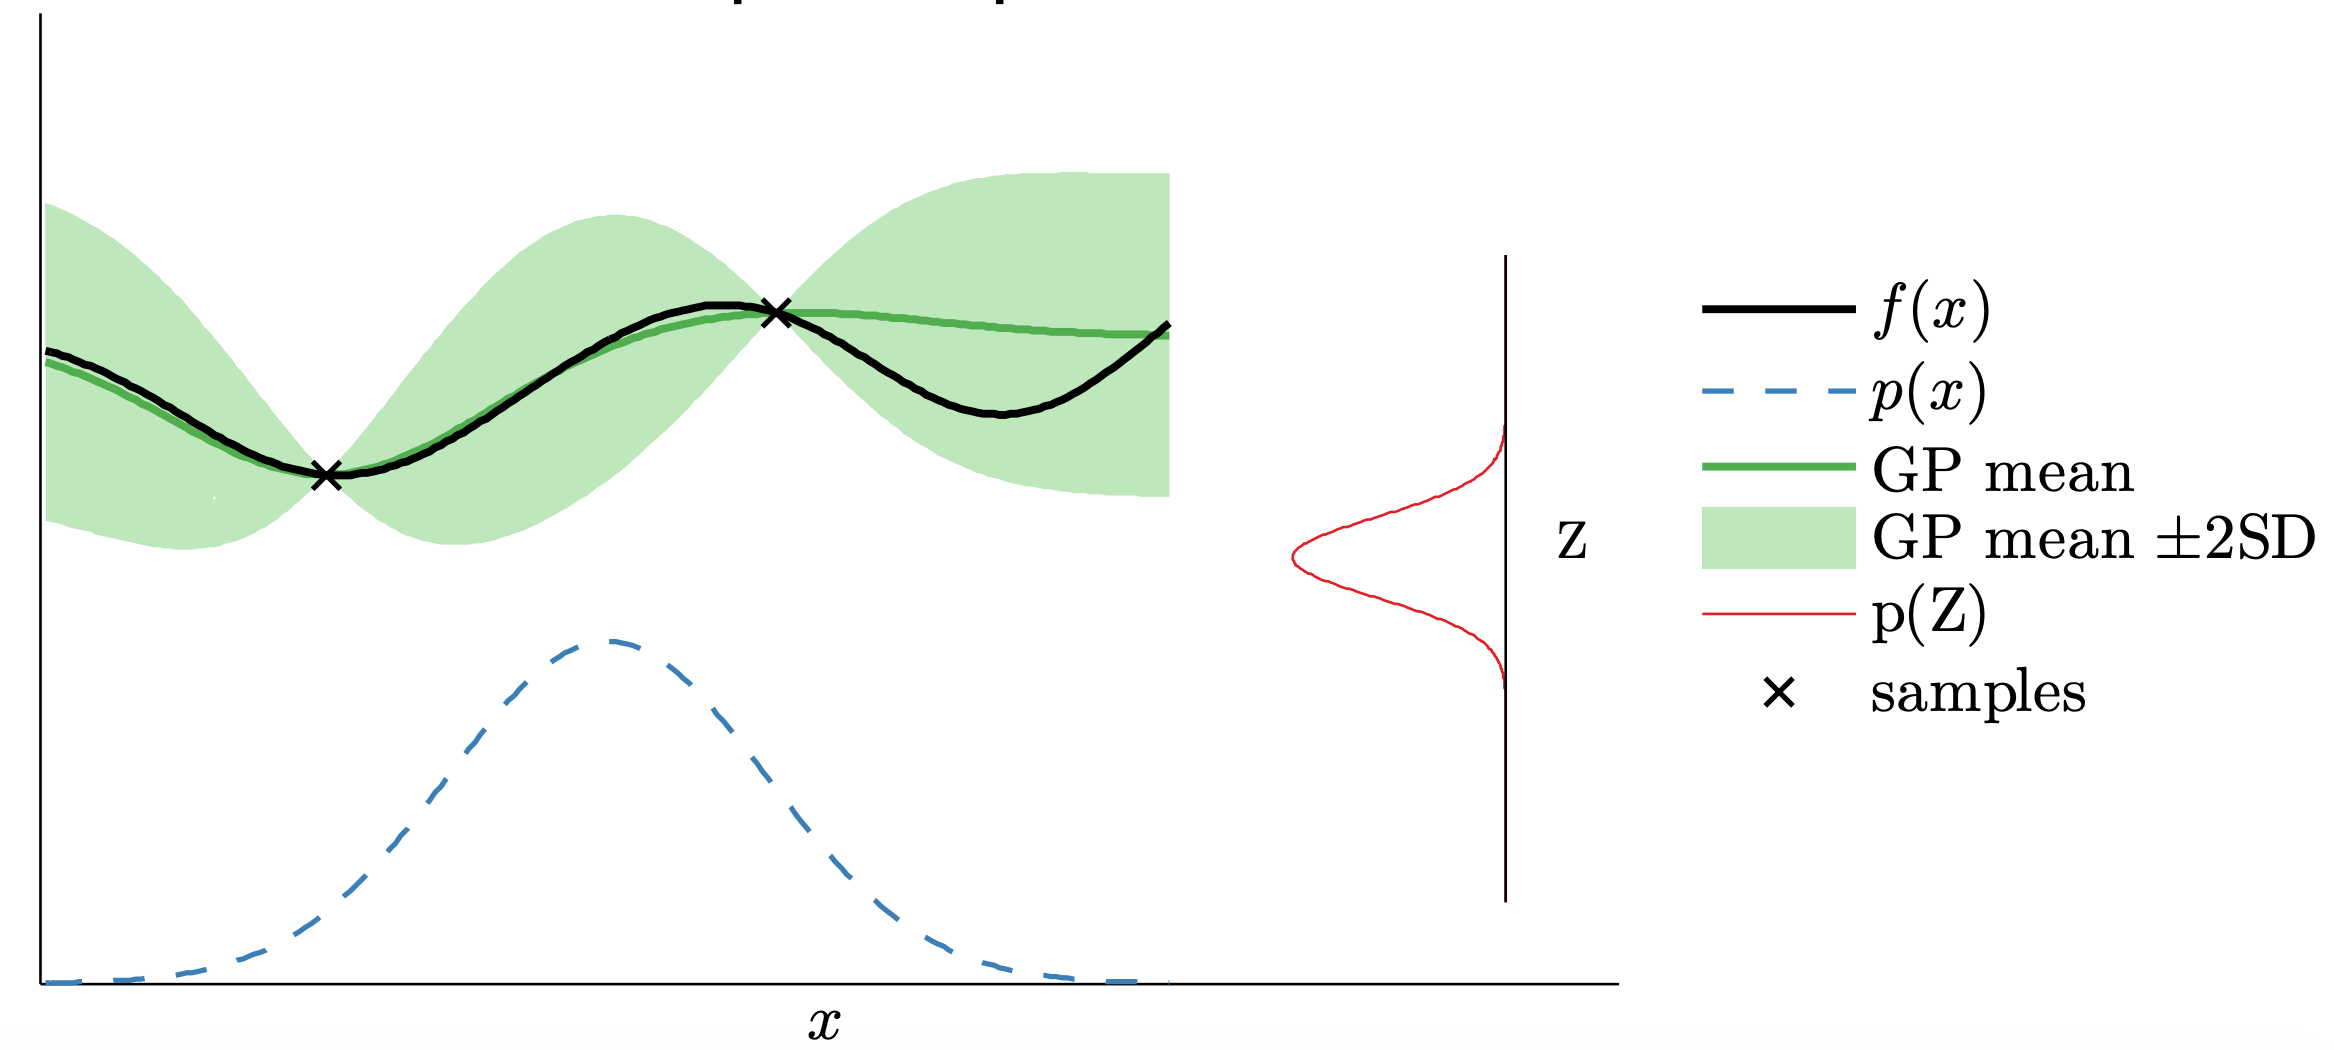
\includegraphics[scale=.33]{bq.png}
\caption{\textbf{An illustration of Bayesian Quadrature.}\\\textit{Source:} \cite{huszar}}
\label{fig:bq}
\end{figure}

First of all, let's determine the conditional distribution $\displaystyle
 p[f]| \; \mathbf{f}$ where
$\mathbf{f} = \transpose{\prt{f_1, \ldots, f_n}}$.
Since both $p[f]$ and $\mathbf{f}$ are gaussian, we can use the conditional gaussian rule:
\begin{boxdefinition}
  By denoting, $y_1 := p[f]$, $y_2 = \mathbf{f}$, $y = \begin{pmatrix}
    y_1\\y_2
\end{pmatrix}$, $\displaystyle \Sigma = \begin{pmatrix}
  \Sigma_{1,1}, \Sigma_{1,2}\\
  \Sigma_{2,1}, \Sigma_{2,2}
\end{pmatrix}$ its covariance matrix by blocks, we have :
$$p[f]| \; \mathbf{f} \sim \mathcal { N } (  \mu  , \Stilde )$$
where

  %
  %

  \begin{equation*}
  \begin{cases}
    \mu \;&= \;  \Sigma _ { 12 } \; \Sigma _ { 22 } ^ { - 1 } \; \mathbf{f} \\
     \Stilde \; &= \;  \Sigma _ { 11 } \;- \Sigma _ { 12 } \;\Sigma _ { 22 } ^ { - 1 } \; \Sigma _ { 21 }.
  \end{cases}
\end{equation*}
\end{boxdefinition}

Let's determine what $\mu$ and $\Stilde$ look like in our context.
  \begin{boxcomputation}
\begin{align*}
  \Sigma _ { 22 } &= \prt{\Cov{f_i}{f_j}}_{1 \leq i,j \leq n}\\
  &= \prt{\Cov{f(x_i)}{f(x_j)}}_{1 \leq i,j \leq n}\\
  &= \prt{k(x_i, x_j)}_{1 \leq i,j \leq n}\\
  &= K\\
  \mu &= \begin{pmatrix}
    \Cov{p[f]}{f_1} \\ \ldots \\ \Cov{p[f]}{f_n}\\
\end{pmatrix} K^{-1} \mathbf{f}
\end{align*}
\end{boxcomputation}
Let's rewrite the vector from the left:
\begin{boxcomputation}
\begin{align*}
\Cov{p[f]}{f_i} &= \int_{\Omega} p[f](w) f(x_i, w) \d \P(w)\\
&= \int_{\Omega} \int_{\X} f(x, w) \d \mu(x) f(x_i, w) \d \P(w)\\
&=  \int_{\X}  \underbrace{\int_{\Omega} f(x, w) f(x_i, w) \d \P(w)}_{=\Cov{f(x)}{f(x_i)}=k(x,x_i)} \d \mu(x) \\
&= \int_{\X} k(x,x_i)\d \mu(x)\\
&= \int_{\X} \Phi(x_i)(x) \d \mu(x)\\
&= p[\Phi(x_i)]\\
&= \mu_p \prt{x_i}\\
\end{align*}
\end{boxcomputation}

By denoting $z := \prt{z_i}_{i=1}^n = \prt{\mu_p \prt{x_i}}_{i=1}^n \in \R^n$, we
 get the desired formula\footnote{formula 4 in \cite{FWBQ} } for the expectation:
 \begin{boxtheorem}
   \begin{equation}
     \mu = z ^ { T } K ^ { - 1 } \mathbf { f }
   \end{equation}
 \end{boxtheorem}

The variance is then straightforward :
\begin{boxexample}
  \begin{align*}
    \Stilde &= \Var{p[f]} - z ^ { T } K ^ { - 1 } z\\
    &= \int_{\X^2}  k(x,y) \d \mu(x) \d \mu(y) - z ^ { T } K ^ { - 1 } z
  \end{align*}
\end{boxexample}

\begin{boxcomputation}
  We need to simplify the integral to obtain the desired formula for the variance:
\begin{align*}
  \int_{\X^2}  k(x,y) \d \mu(x) \d \mu(y) &= \int_{\X} \int_{\X} \Phi(x)(y) \d \mu(y) \d \mu(x) \\
  &= \int_{\X} p[\Phi(x)] \d \mu(x) \\
  &= \int_{\X} \mu_p\prt{x} \d \mu(x) \\
  &=  p[\mu_p]
\end{align*}
\end{boxcomputation}
which leads us to the desired result:
\begin{boxtheorem}
  $$\Stilde = p[\mu_p] -z ^ { T } K ^ { - 1 } z$$
\end{boxtheorem}

Both the conditional expectation and variance are essentials in the FWBQ\footnote{Frank-Wolfe Bayesian Quadrature} algorithm:
\begin{itemize}[font= \color{blue} \large, label= $\bullet$]
  \item $\mu = z ^ { T } K ^ { - 1 } \mathbf { f }$ which can be written as
  $\displaystyle \mu = \sum_{i=1}^n w_i^{BQ} f_i$ where $w^{BQ} := \transpose{\prt{K^{-1}}}z$. $\mu$ appears to be the \textbf{most natural estimation of our integral} $p[f]$.
  It also gives us the \textbf{new weights to update}.
  \item $\Stilde = p[\mu_p] -z ^ { T } K ^ { - 1 } z$ which is also equal to $\MMD^2$
  according to \cite{huszar} and can be interpreted as our \textbf{uncertainty}. Therefore
  we need to \textbf{choose $\acc{x_i}$ which minimize this quantity}. This will be achieved
  by using the Frank Wolfe algorithm described in the next section.
\end{itemize}

% Conditional rule demonstrated
% Demonstration formula 4
% Demonstration formula 5

\section{Frank-Wolfe algorithm}
\label{sec:FW}

Let's $J$ be a convex differentiable real-valued function on a
domain $\G\subset\H$ which is supposed to be a compact and convex.

The Frank-Wolfe algorithm \cite{fwalgo} proposes a method to solve the following optimization
 problem :

\begin{boxproblem}
  \begin{equation} \label{eq:fwpbm}
    \begin{array} { l } { \text { Minimize } \acc{J ( \mathbf { x } )} } \\ { \text { subject to } \mathbf { x } \in \G } \end{array}
  \end{equation}
\end{boxproblem}
Let's describe here both the Frank-Wolfe algorithm and its variant with the Line Search :
\begin{boxprogramming}
\begin{mydescription}
  \item [Initialization] $g _ { 1 } = \overline { g } _ { 1 } \in \mathcal { G }$ and
  step-size sequence $\acc{\rho_i}_{i=1}^n$ (not required in the FWLS algorithm).
  \item [Iterations] For $i=2$ to $n$ :
  \begin{mydescription}[0.2cm]
    \item [Search direction] we replace in \eqref{eq:fwpbm} $J$ by its first-order
    Taylor expansion around $g_k$ to solve the following subproblem :
      \begin{equation}\label{eq:fwlin}
        \begin{array} { c } { \text { minimize }  \acc{J \left( g_{i-1} \right) + \nabla J \left( g_{i-1} \right) ^ { \mathrm { T } } \left( g - g_{i-1} \right)} } \\ { \text { subject to } g \in \G } \end{array}
      \end{equation}
Let's denote as \cite{FWBQ}
\begin{equation}\label{eq:gbar}
  \overline { g } _ { i } := \arg \min _ { g \in \G } \bigps{g}{ \nabla J \left( g _ { i - 1 } \right)}
\end{equation}
 where we have removed
 in \eqref{eq:fwlin} terms independent of the optimization variable.
 \item [New iteration point]: we choose $g_i$ as a \textit{convex}-combination of
 $g_{i-1}$ and $\overline{g_i}$.
 \begin{equation}
   \label{eq:12}
   g _ { i } = \left( 1 - \rho _ { i } \right) g _ { i - 1 } + \rho _ { i } \overline{ g } _ { i }
 \end{equation}
 \begin{mydescription}
\item [FW] $\rho _ { i }$ is  determined by the sequence given at the initialization
\item [FWLS]
\begin{equation*}
\rho _ { i } := \operatorname { argmin } _ { \rho \in [ 0,1 ] } J \left( ( 1 - \rho ) g _ { i - 1 } + \rho \overline{g _ { i }} \right)
\end{equation*}

 \end{mydescription}
  \end{mydescription}
\end{mydescription}
\end{boxprogramming}

\begin{tikzpicture}[line cap=round,line join=round,>=triangle 45,x=1cm,y=1cm]
\clip(-9,-4) rectangle (0.24,2);
\fill[line width=2pt,color=ggyellow,fill=ggyellow,fill opacity=0.10000000149011612] (-5.58,1.24) -- (-3.52,1.34) -- (-1.08,-1.24) -- (-4.38,-3.46) -- (-8.1,-2.2) -- cycle;
\draw [color=ggyellow] (-5.58,1.24)-- (-3.52,1.34);
\draw [color=ggyellow] (-3.52,1.34)-- (-1.08,-1.24);
\draw [color=ggyellow] (-1.08,-1.24)-- (-4.38,-3.46);
\draw [color=ggyellow] (-4.38,-3.46)-- (-8.1,-2.2);
\draw [color=ggyellow] (-8.1,-2.2)-- (-5.58,1.24);
\draw [->] (-4.42,-0.94) -- (-3.02,-0.1);
\draw [dotted] (-4.42,-0.94)-- (-7.29,-2.47);
\draw [dotted] (-4.42,-0.94)-- (-8.1,-2.2);
\draw [->] (-5.73,-1.38) -- (-4.42,-1.84);
\draw [dotted] (-5.41,-1.47)-- (-7.10,-0.84);
  \node[draw] at (-3.02,0.3)  (grad1) {$\mathbf{\nabla J(g_1)}$};
  \node[draw] at (-4.22,-2.3)  (grad2) {$\mathbf{\nabla J(g_2)}$};
\draw [fill=blue] (-4.42,-0.94) circle (2pt) node[below] {$\mathbf{g_1}$};
\draw [fill=blue] (-8.1,-2.2) circle (2pt) node[shift={(-1.5ex,-2ex)}] {$\mathbf{\overline{g_2}=\overline{g_3}}$};
\draw [fill=blue] (-5.73,-1.38) circle (2pt) node[shift={(0ex,-2.5ex)}] {$\mathbf{g_2}$};
\draw [fill=blue] (-6.32,-1.59) circle (2pt) node[shift={(-0.5ex,2ex)}] {$\mathbf{g_3}$};
\draw[->,ggred, looseness=2] (-4.42,-0.94) .. controls (0,-2.3) and  (-4,-4.5) .. node[sloped] {} (-8.1,-2.2);
\draw[->,ggred] (-8.1,-2.2) -- (-5.73,-1.38);
\draw[->,ggred, looseness=2] (-5.73,-1.38) .. controls (-5.6,0.5) .. node[sloped] {} (-8.1,-2.2);
\draw[->,ggred] (-8.1,-2.2) -- (-6.32,-1.59);
\end{tikzpicture}
\begin{center}
  \textbf{An illustration of the Frank Wolfe algorithm. }
\end{center}
  In equation \eqref{eq:gbar}, we don't have necessarily $\overline{g_i} \in \spn{\nabla J(g_{i-1})}$. In fact, we can clearly see in the illustration above
   that the point
   \begin{align*}
  \widetilde { g } _ { i } &:= \arg \min _ { g \in \G\cap  \spn{\nabla J(g_{i-1})}} \bigps{g}{ \nabla J \left( g _ { i - 1 } \right)} \\
  &= \arg \min _ { \alpha \geq 0}
  \acc{-\alpha \nabla J(g_{i-1}) \mid \alpha \nabla J(g_{i-1}) \in \G}
\end{align*}
would not be optimal as
\begin{equation*}
  \inner{\overline { g } _ { i }}{\nabla J(g_{i-1})}
  < \inner{\widetilde { g } _ { i }}{\nabla J(g_{i-1})}.
\end{equation*}



% \hspace{-1.5cm}
\begin{tikzpicture}[line cap=round,line join=round,>=triangle 45,x=1cm,y=1cm]
\clip(-9,-4) rectangle (0.24,2);
\fill[line width=2pt,color=ggyellow,fill=ggyellow,fill opacity=0.10000000149011612] (-5.58,1.24) -- (-3.52,1.34) -- (-1.08,-1.24) -- (-4.38,-3.46) -- (-8.1,-2.2) -- cycle;
\draw [color=ggyellow] (-5.58,1.24)-- (-3.52,1.34);
\draw [color=ggyellow] (-3.52,1.34)-- (-1.08,-1.24);
\draw [color=ggyellow] (-1.08,-1.24)-- (-4.38,-3.46);
\draw [color=ggyellow] (-4.38,-3.46)-- (-8.1,-2.2);
\draw [color=ggyellow] (-8.1,-2.2)-- (-5.58,1.24);
\draw [->] (-4.42,-0.94) -- (-3.02,-0.1);
\draw [dotted] (-4.42,-0.94)-- (-7.29,-2.47);
\draw [->] (-5.41,-1.47) -- (-4.42,-1.84);
\draw [dotted] (-5.41,-1.47)-- (-7.10,-0.84);
  \node[draw] at (-3.02,0.3)  (grad1) {$\mathbf{\nabla J(g_1)}$};
  \node[draw] at (-4.22,-2.3)  (grad2) {$\mathbf{\nabla J(g_2)}$};
\draw [fill=blue] (-4.42,-0.94) circle (2pt) node[below] {$\mathbf{g_1}$};
\draw [fill=blue] (-7.294,-2.47) circle (2pt) node[shift={(-1.5ex,-1.5ex)}] {$\mathbf{\widetilde{g_2}}$};
\draw [fill=blue] (-5.41,-1.47) circle (2pt) node[shift={(0ex,-2.5ex)}] {$\mathbf{g_2}$};
\draw [fill=blue] (-7.10,-0.846) circle (2pt) node[shift={(-1.5ex,1.5ex)}] {$\mathbf{\widetilde{g_3}}$};
\draw [fill=blue] (-6.01,-1.246) circle (2pt) node[shift={(0ex,2.5ex)}] {$\mathbf{g_3}$};
\draw[->,ggred, looseness=2] (-4.42,-0.94) .. controls (0,-2.3) and  (-4,-4.5) .. node[sloped] {} (-7.29,-2.47);
\draw[->,ggred] (-7.29,-2.47) -- (-5.41,-1.47);
\draw[->,ggred, looseness=2] (-5.41,-1.47) .. controls (-5.6,0.5) .. node[sloped] {} (-7.10,-0.846);
\draw[->,ggred] (-7.10,-0.846) -- (-6.01,-1.246);
\end{tikzpicture}
\begin{center}
  \textbf{Comparison with a descent algorithm. }
\end{center}

Another important fact of the Frank Wolfe algorithm is that the output $g_n$
can easily be expressed as a linear combination of atoms $\overline{g_i}$.

In fact we have the following formula, which corresponds to the equation (\textcolor{electriccrimson}{7}) in \cite{FWBQ}:
\begin{boxtheorem}
  For all $n \geq 2$ :
  \begin{equation}
    \label{eq:13}
    g_n = \sum_{k=1}^n \underbrace{ \rho_k \acc{\prod_{k<i\leq n} (1-\rho_i)} }_{:=w_k^{FW}} \cdot \overline{g_k} = \sum_{k=1}^n w_k^{FW}\cdot \overline{g_k}
  \end{equation}
  with $\rho_1 = 1$.
\end{boxtheorem}

The formula in \cite{FWBQ} is slightly different :
\begin{equation*}
  g _ { n } = \sum _ { i = 1 } ^ { n } \rho _ { i - 1 }\acc{ \prod _ { j = i + 1 } ^ { n } \left( 1 - \rho _ { j - 1 } \right) } \cdot \overline { g } _ { i }
\end{equation*}
with $\rho_0=1$ but clearly doesn't work. In fact according to the algorithm, by taking $n=2$ we should have :
\begin{equation*}
  g_2 = (1-\rho_2) \cdot \overline{g_1} + \rho_2 \cdot \overline{g_2}
\end{equation*}
while their formula gives
\begin{align*}
  g _ { 2 } &= \sum _ { i = 1 } ^ { 2 } \rho _ { i - 1 }\acc{ \prod _ { j = i + 1 } ^ { 2 } \left( 1 - \rho _ { j - 1 } \right) } \overline { g } _ { i }\\
  &= (1-\rho_1) \cdot  \overline{g_1}+\rho_1 \cdot \overline{g_2}.
\end{align*}
Let's prove \eqref{eq:13} by induction.

\begin{boxcomputation}
\begin{mydescription}
  \item [Base case]: $n=2$. Our formula gives :
  \begin{align*}
    g_2 &= \sum_{k=1}^2  \rho_k \acc{\prod_{k<i\leq 2} (1-\rho_i)} \cdot \overline{g_k}\\
    &= (1-\rho_2) \cdot \overline{g_1}+ \rho_2 \cdot \overline{g_2}
  \end{align*}
  as we have set $\rho_1 = 1$, as expected.
  \item [Step case]: Assume the formula holds for $n-1$ and let's prove it for $n$.
  Using the recurrence relation of \eqref{eq:12} and our assumption, we have :
  \begin{align*}
    g _ {n} &= \left( 1 - \rho _ {n} \right) \cdot g _ {n- 1 } + \rho _ {n} \cdot \overline { g } _ {n}\\
    &= \left( 1 - \rho _ { n } \right) \cdot \sum_{k=1}^n \rho_k \acc{\prod_{k<i\leq n-1} (1-\rho_i)} \cdot \overline{g_k} + \rho_n \cdot \overline { g } _ {n}\\
    &= \sum_{k=1}^n \rho_k \acc{\prod_{k<i\leq n} (1-\rho_i)} \cdot \overline{g_k} + \rho_n\cdot \overline { g } _ {n}\\
    &= \sum_{k=1}^n \rho_k \acc{\prod_{k<i\leq n} (1-\rho_i)}  \cdot \overline{g_k}
  \end{align*}
  which ends the proof.
\end{mydescription}
\end{boxcomputation}

It is common to take harmonic coefficients in the standard FW algorithm\footnote{Let's remember that in the FWLS algorithm, $\acc{\rho_i}$ and thus $\acc{w_k^{FWLS}}$ are
determind by the line search step.} as a choice for $\acc{\rho_i}:= \acc{\frac{1}{i}}_{i=1}^n$,
 which gives us uniform weights as showed bellow :
 \begin{align*}
w_k^{FW} &= \frac{1}{k} \acc{\prod_{k<i\leq n} \prt{1-\frac{1}{i}}}= \frac{1}{k} \cdot \frac{k}{n} = \frac{1}{n}.
\end{align*}

Let's set here the framework of our optimization problem.

\begin{boxproblem}
  We want to approximate the mean element $\mu_p$ with a linear combination of
  elements of the form :$$\Phi(x)= k\prt{\cdot\;,\; x}.$$
  In fact, let's say we have:
   $$\mu_p \approx \hat{\mu_p} := \sum_{k=1}^n w_k \Phi(x_k).$$
   Using the reproducing property, we will then have :
   $$\hat{p}[f]= \bigps{f}{\mu_p} = \sum_{k=1}^n w_k f(x_k),$$
   which is a quadrature rule.

   In order to do this, let's assume that we optimize the following convex function :
   \begin{equation}
     J(g):= \frac{1}{2} \norme{g-\mu_p}^2
   \end{equation}
on the domain $\G \subseteq \H$ where $\G$ refers to the closure of the convex hull
of $\Phi\prt{\X}$, which is assumed to be uniformly bounded, \ie
\begin{equation*}
  \exists R > 0 : \forall x \in \mathcal { X } , \| \Phi ( x ) \| _ { \mathcal { H } } \leq R
\end{equation*}

\end{boxproblem}
But a question rises : Why atoms $g_i$ should be of the form $\Phi(x_i)$?

In fact, let's
 $g$ be a point in the domain. Because of its definition,
  $g$ can simply be expressed as a convex combination of elements in the feature space $\Phi(\X)$, \ie $g = \sum_k \alpha_k \Phi(x_k)$ with $\sum_k \alpha_k=1$ and thus we have :
 \begin{align*}
   \bigps{g}{\grad{J}(g_{i-1})} &= \sum_k \alpha_k \cdot \bigps{\Phi(x_k)}{\grad{J}(g_{i-1})}\\
   &\geq \prt{\sum_k \alpha_k} \cdot \min_{k} \bigps{\Phi(x_k)}{\grad{J}(g_{i-1})}\\
   &= \bigps{\Phi(x_{k_0})}{\grad{J}(g_{i-1})}
 \end{align*}
 for $k_0$ such that $k_0 \in \argmin{\bigps{\Phi(x_k)}{\grad{J}(g_{i-1})}}$.

 We now understand how can the Frank Wolfe algorithm be useful here : because the
 minimization of \eqref{eq:gbar} can be restricted at extreme points of the domain,
 selecting atoms of the form $\Phi(x_k)$ allow us to select interesting points $\acc{x_k}$ which are needed for the bayesian quadrature which are solution of the
 following optimization problem :
 \begin{equation}
   x_k \in \arg \min _ { x \in \mathcal { X } } \left\langle \Phi ( x ) , g _ { k - 1 } - \mu _ { p } \right\rangle _ { \mathcal { H } }
 \end{equation}
 where $g \in \G$ in the left term of the inner product has been replaced by $\Phi(x) \in \G$ with $x \in \X$.

 Therefore, if we denote by $\acc{w_l}_{l=1}^{i-1}$ the coefficients in front of
 $\acc{\Phi(x_l)}_{l=1}^{i-1}$ in $g_{i-1}$ and using the reproducing kernel property, we have :
 \begin{align*}
   \left\langle \Phi ( x ) , g _ { i - 1 } - \mu _ { p } \right\rangle _ { \mathcal { H } } &= \left\langle \Phi ( x ) , \sum _ { l = 1 } ^ { i - 1 } w _ { l } ^ { ( i - 1 ) } \Phi \left( x _ { l } \right) - \mu _ { p } \right\rangle _ { \mathcal { H } }\\
   &= \sum _ { l = 1 } ^ { i - 1 } w _ { l } ^ { ( i - 1 ) } k \left( x , x _ { l } \right) - \mu _ { p } ( x )\\
 \end{align*}
which gives an explicit formula for the optimization problem\footnote{We remark that if
 the optimization problem on $g \in \G$ was a classic convex problem, this is not the case anymore when we perform the optimization on $x \in \X$.} with known quantities.
 In fact, in the simulations that we have been able to reproduce successfully, the choice of a gaussian kernel $k$ allow us to compute $\mu_p( \cdot )$ easily. See \cite{FWBQ} \textit{Appendix C} for more details.
 \section{The Frank-Wolfe Bayesian Quadrature algorithm}
 \label{sec:CC}

We describe here the final algorithm which is a combination of the two previous
 ones.
    At each iteration \texttt{i}:
 \begin{mydescription}
   \item [Selecting a new $x_i$] through the Frank Wolfe algorithm with $g_{i-1}$ depending
   on the BQ weights of the iteration \texttt{i-1} and FW design points of all previous iteration \texttt{j} with $1 \leq j<i$.
   \item [Selecting new weights $\acc{w_k^{BQ}}_{k=1}^i$] with the bayesian quadrature.
 \end{mydescription}

 It's important to note that weights at each iteration \texttt{i} are used only for
 the next iteration \texttt{i+1} while the design points $x_i$ are used for all iteration \texttt{j} with $i<j\leq n$.

\section{Consistency}
\label{sec:consistency}

We will establish here the main result of the article \cite{FWBQ} and referred as Theorem 1:
\begin{boxdefinition}
  \begin{center}
    \textit{The posterior mean }$\hat { p } _ { \mathrm { FWBQ } } [ f ]$ \textit{converges
    to the true integral }$p[f]$ at the following rates:
  \end{center}
\begin{align}
    \left| p [ f ] - \hat { p } _ { \mathrm { FWBQ } } [ f ] \right| &\leq M M D \left( \left\{ x _ { i } , w _ { i } \right\} _ { i = 1 } ^ { n } \right) \nonumber\\
    &\leq \left\{ \begin{array} { c c } { \frac { 2 D ^ { 2 } } { R } n ^ { - 1 } } & { \footnotesize \text {for  FWBQ} } \\ { \sqrt { 2 } D \exp \left( - \frac { R ^ { 2 } } { 2 D ^ { 2 } } n \right) } & {\footnotesize \text {for FWLSBQ } } \end{array} \right.
\end{align}
where the FWBQ uses step-size $\rho _ { i } = 1 / ( i + 1 )$, $D \in ( 0 , \infty )$
  is the diameter of the marginal polytope $\G$ and $R \in ( 0 , \infty )$ gives the
  radius of the \textbf{largest}\footnote{There was a typo here in \cite{FWBQ} as the authors mentioned the radius  of the smallest ball which is clearly zero. In fact, greater is the radius and better is the inequality, so of course we are more interested in large
  radius rather than smaller ones. } ball of center $\mu_p$ included in $\G$.
\end{boxdefinition}

It was a bit disappointing to see that the authors of \cite{FWBQ} did not prove the most interesting part of the theorem,
 which is the introduction of the diameter of the marginal polytope ($D$) and the radius of the largest ball of center $\mu_p$ ($R$). Instead, it came out of nowhere quoting \cite{Bach}, which is of course deeply unsatisfactory from a scientific standpoint
  as it gives no clear understanding about the intuition behind this result.

  We were able to find more details about this result in \cite{Beck} and \cite{Chen}.
Let's start assuming as \cite{Bach} that $\mu_p$ is in the relative interior
of $\G$ :
\begin{equation}
\exists r>0 \text{ such that } B(\mu_p, r) \subset \G.
\end{equation}



We start with a proposition\footnote{Proposition 3.1 in \cite{Beck}.} :
\begin{boxtheorem}
  We denote by $R$ the radius of the largest ball of center $\mu_p$.
  Using the same notations as previously and the assumption above, we have at
  iteration \texttt{i+1}:
  \begin{equation}
    \Bigps{\mu_p-g_{i}}{\mu_p-\overline{g_{i+1}}}+R \norme{\mu_p-g_{i}} \leq 0
  \end{equation}
\end{boxtheorem}

\begin{boxcomputation}
  By denoting $d = \mu_p-g_i$ and using the definition of $R$ we have :
\begin{equation*}
  g = \mu_p+R\cdot \frac{d}{\norme{d}} \in \G.
\end{equation*}
Moreover by using the definition of $\overline{g_{i+1}}$ we get:
  \begin{align*}
\Bigps{\mu_p-g_{i}}{\mu_p-\overline{g_{i+1}}} &=
\Bigps{-\grad{J(g_i)}}{\mu_p-\overline{g_{i+1}}}\\&\leq
\Bigps{-\grad{J(g_i)}}{\mu_p-g}\\
&\leq R\cdot\Bigps{\mu_p-g_{i}}{\frac{d}{\norme{d}}}\\
&\leq -R \norme{d}
  \end{align*}
  which is the desired result.
\end{boxcomputation}




\section{Contraction}
\label{sec:contraction}


\section{Experimental Results}
\label{sec:ER}

\subsection{Overview of the code}

We have implemented the following algorithms : -- FW and FWBQ (when Line-Search mode is disabled) -- FWLS and FWLSBQ (when Line-Search mode is enabled). Two notebooks are available. The first notebook applies the different algorithms to a simulation study. The second notebook is an example of how the algorithms can be used to solve a problem in a specific area.

\subsection{Simulation Study}

We also used an exponentiated-quadratic (EQ) kernel $k(x, x') := \lambda^{2} exp(-\frac{1}{2}\sigma^{2} \| x-x' \|_{2}^{2} )$. EQ kernel is a relevant choice when $p$ is a mixture of gaussians. Moreover, the mean element $\mu_{p}$ has a closed-form expression.
In order to replicate the simulation study of the paper, we took $p$ as a mixture of 20 two-dimensional gaussians. Two dimensions for each gaussians allow us to plot selected points, the function $f$, the approximation of the mean element $g_n$ and the mean element $\mu_{p}$ so that we can come up with a visual representation of the algorithms.

\subsection{An example of application}

% intuition
% graph to show that it is closed to a gradient descent
% drawing line search Aspremont

\section*{Resources}
\label{sec:bibli}

\nocite{*}
\printbibliography[heading=none]
